%% beamerthemeImperialPoster v1.0 2016/10/01
%% Beamer poster theme created for Imperial College by LianTze Lim (Overleaf)
%% LICENSE: LPPL 1.3
%%
%% This is the example poster demonstrating use
%% of the Imperial College Beamer Poster Theme
\documentclass[xcolor={table}]{beamer}
%% Possible paper sizes: a0, a0b, a1, a2, a3, a4 (although Imperial College posters are usually A0 or A1).
%% Possible orientations: portrait, landscape
%% Font sizes can be changed using the scale option.
\usepackage[size=a1,orientation=landscape,scale=1.55]{beamerposter}

\usetheme{ImperialPoster}

%% Four available colour themes
\usecolortheme{ImperialWhite} % Default
% \usecolortheme{ImperialLightBlue}
% \usecolortheme{ImperialDarkBlue}
% \usecolortheme{ImperialBlack}

\title{$11^{th}$ International Summer School on Geometry, Mechanics and Control - Participant's Thumbnail Academic Biography}

\author{\ \mainauthor{Nader Ganaba}\Tsup{1}}

\institute{\Tsup{1}Department of Mathematics, Faculty of Natural Sciences, Imperial College London.}

%\addbibresource{refs.bib}


\begin{document}
\begin{frame}[fragile=singleslide,t]\centering

\maketitle

\begin{columns}[onlytextwidth,T]

%%%% First Column
\begin{column}{.31\textwidth}

\begin{block}{Academic Background}
Nader Ganaba received his B.Sc $(2010)$ in Engineering and Mathematics, control and robotics option, from Queen's University in Kingston (Canada). During that time, he was an active member of Queen's Mostly Autonomous Sailboat Team (QMAST), a competitive engineering team, and in his senior year he was the lead programmer. In $2014$, he obtained an M.Sc in applied mathematics from Imperial College London. He is currently a PhD student, supervised by Prof. Darryl Holm, at Imperial College London. 
\end{block}

\begin{block}{Research Interests}
\begin{description}[align=left]
\item [Nonlinear stability of stochastic dynamical systems] In \cite{arnaudon2017stochastic}, the stochastic energy-Casimir method is presented. The method was developed primarily to study the nonlinear stability of stochastic system.
\item [Stochastic variational integrators] The main topic of research deals with multisymplectic integrators. Also, there is an ongoing work on stochastic Lie-Poisson-Hamilton-Jacobi integrators \cite{G2017}.
\item [Control theory] Three main control problems of interests are: boundary control of partial differential equations, stochastic optimal control problems and numerical optimal control, such as pseudospectral and variational integrators for optimal control. 
\item [Mean field games] It can be used to solve stochastic optimal control problems and it works by solving a system of coupled forward-backward Fokker-Planck and Hamilton-Jacobi-Bellman equations, which can be derived using Clebsch variational principle. 
%\item [High performance computing] Main interest is developing numerical algorithms better suited for distributed systems. Algorithms such as lattice Boltzmann method, smoothed particle hydrodynamics and sparse grids. 
%\item [Evolutionary robotics] The interest in evolutionary robotics stems back from QMAST, and it's a topic rich with interesting problems. Mathematics appears in many areas of ER, such as neural field theory and Inverse optimal control. 
\end{description}


\end{block}
\begin{sidefigure2}
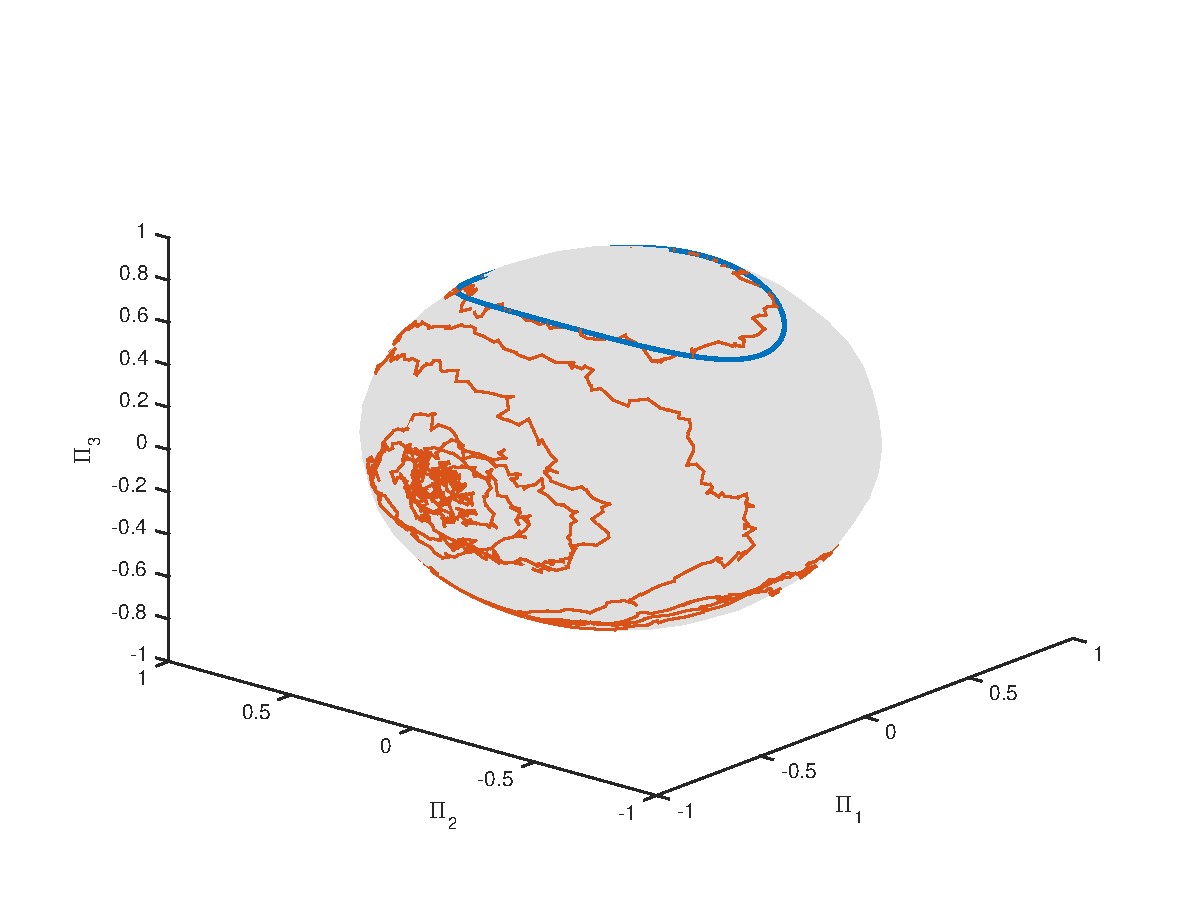
\includegraphics[width=\hsize]{lphj}
\caption{This plot shows the solution of Euler-Poincar\'{e} equation for $\mathrm{SO}(3)$ rigid-body obtained by Lie-Poisson integrator \cite{G2017}. The blue trajectory is the solution of the deterministic equation and the red trajectory is the solution of the stochastic equation. Both equations are solved with the same initial condition. }
\end{sidefigure2}

\end{column}


%%%% Second Column
\begin{column}{.31\textwidth}
\begin{block}{Main Research Topic}
The primary research topic concerns multisymplectic methods for stochastic Euler-Poincar\'{e} for the diffeomorphism group (EPDiff). Motivated by their long time behaviour and their ability to preserve the geometric structure, it is natural to extend such schemes to include stochastic systems. Structure preserving property of the scheme is very important, not just makes the scheme numerically stable, but also physically realistic and preserves conserved quantities.\\
\end{block}


\begin{sidefigureh}
\begin{center}
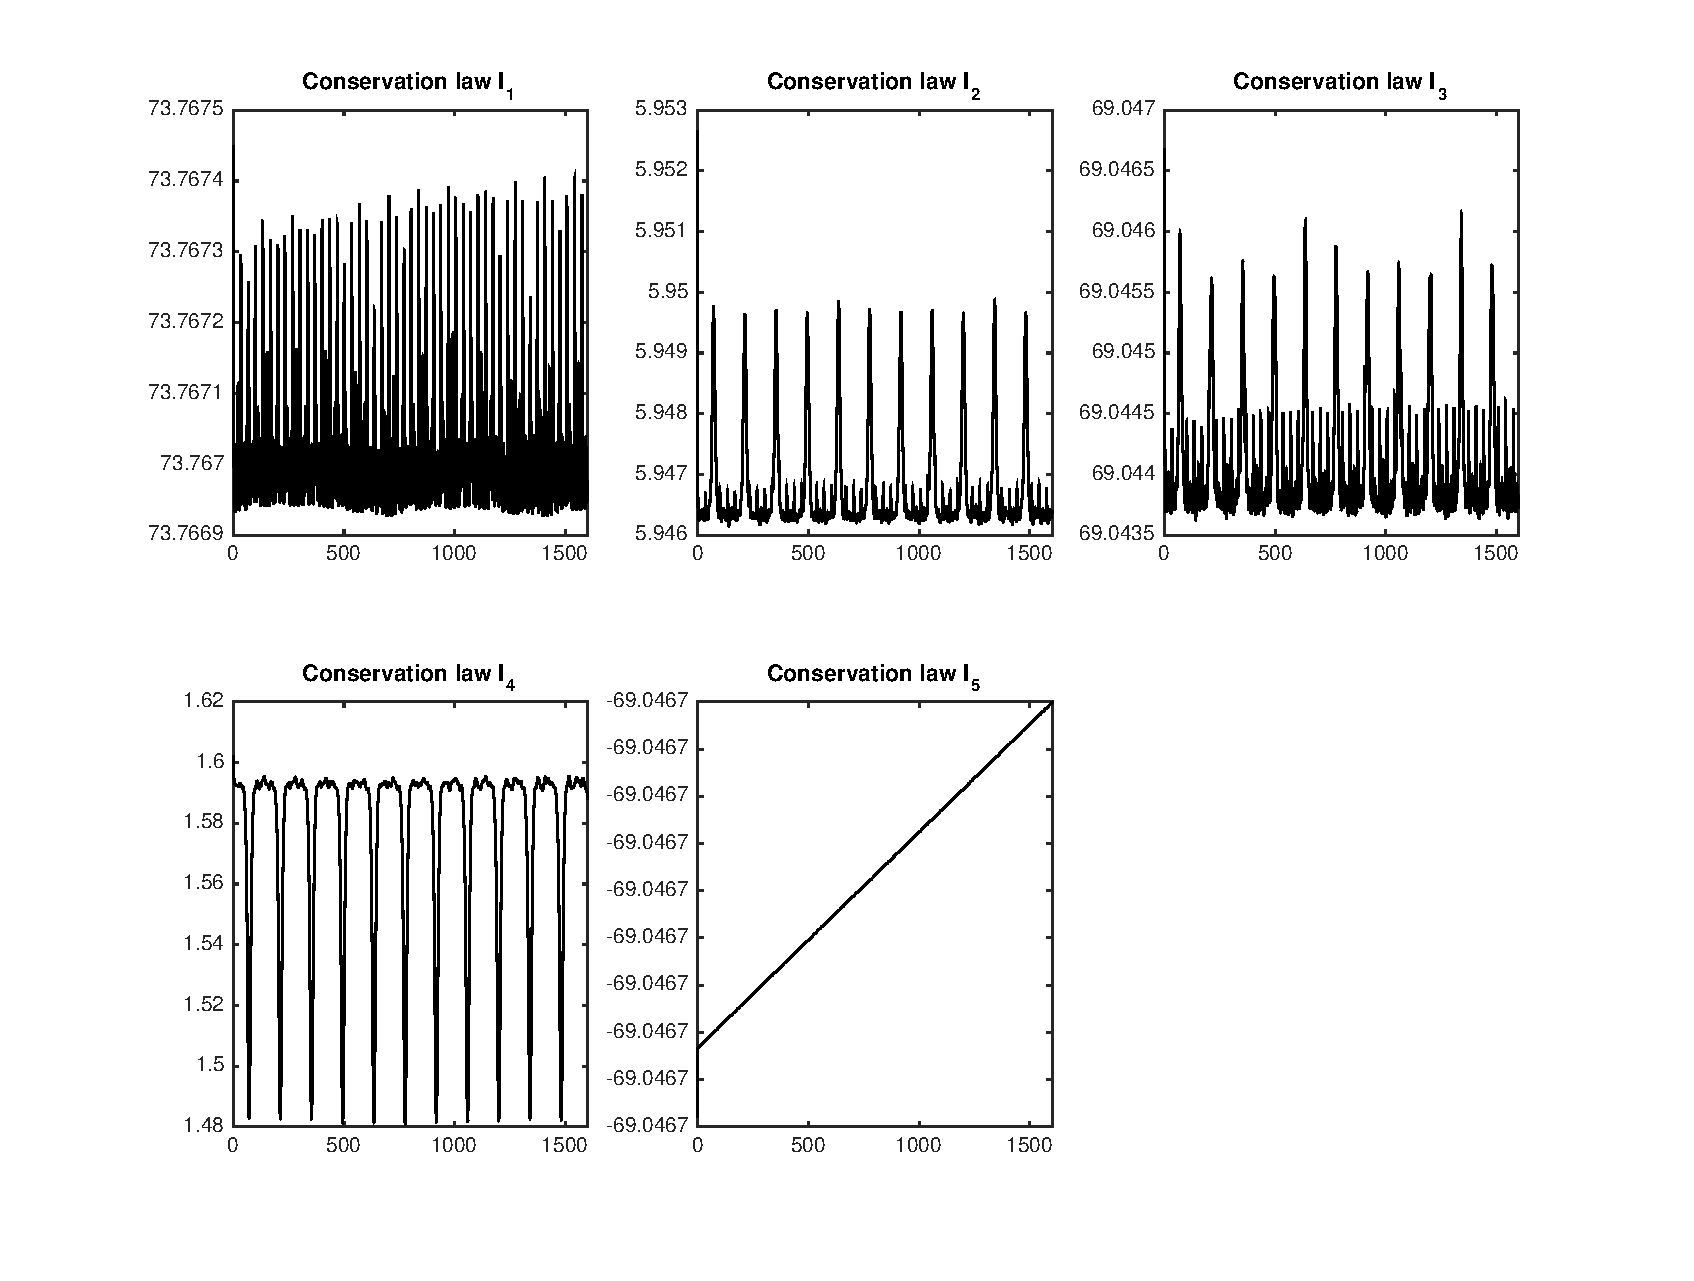
\includegraphics[width=0.9\hsize]{conservation_laws}
\end{center}
\caption{This plot shows the conservation laws of the deterministic Camassa-Holm equation, EPDiff($H^1$), with linear dispersion. The initial condition is chosen to be two solitons with different amplitudes. The simulation was run until $T = 1600$ in a periodic domain, and the waves collided $11$ times during the whole run.}
\end{sidefigureh}


\begin{block}{Clebsch Variational Principle}
\begin{itemize}
\item Clebsch variational principle with back-to-label map is a framework for fluids that yields EPDiff, Euler's equation for ideal fluids, Korteweg-de Vries equation and many others \cite{cotter2007multisymplectic,GHT01}. \\
\item The action functional is
\begin{align*}
\mathbb{S} =\int_0^t \ell(u) \, dt + \left\langle \pi , d_t l +u l_x \, dt \right\rangle + \sum_k \left\langle \pi ,  \xi_k l_x \right\rangle \circ dW_t^k,
\end{align*} \\
\item Using back-to-label map, $l$, allows us to multisymplectic formulation for the
Euler-Poincar\'{e} equation.
%\item The variational principle $ 0 = \delta \mathbb{S}$, yields a set of three stochastic partial differential equations and they are equivalent to the stochastic EPDiff equation
%\begin{align*}
%d_t m + \mathrm{ad}^{\ast}_{u}m \, dt + \sum_k \math,rm{ad}^{\ast}_{\xi_k}m \circ dW_t^k, \quad m = \frac{\delta \ell}{\delta u}
%\end{align*} 
\end{itemize}
\end{block}
,


%\begin{sidefigureh}
%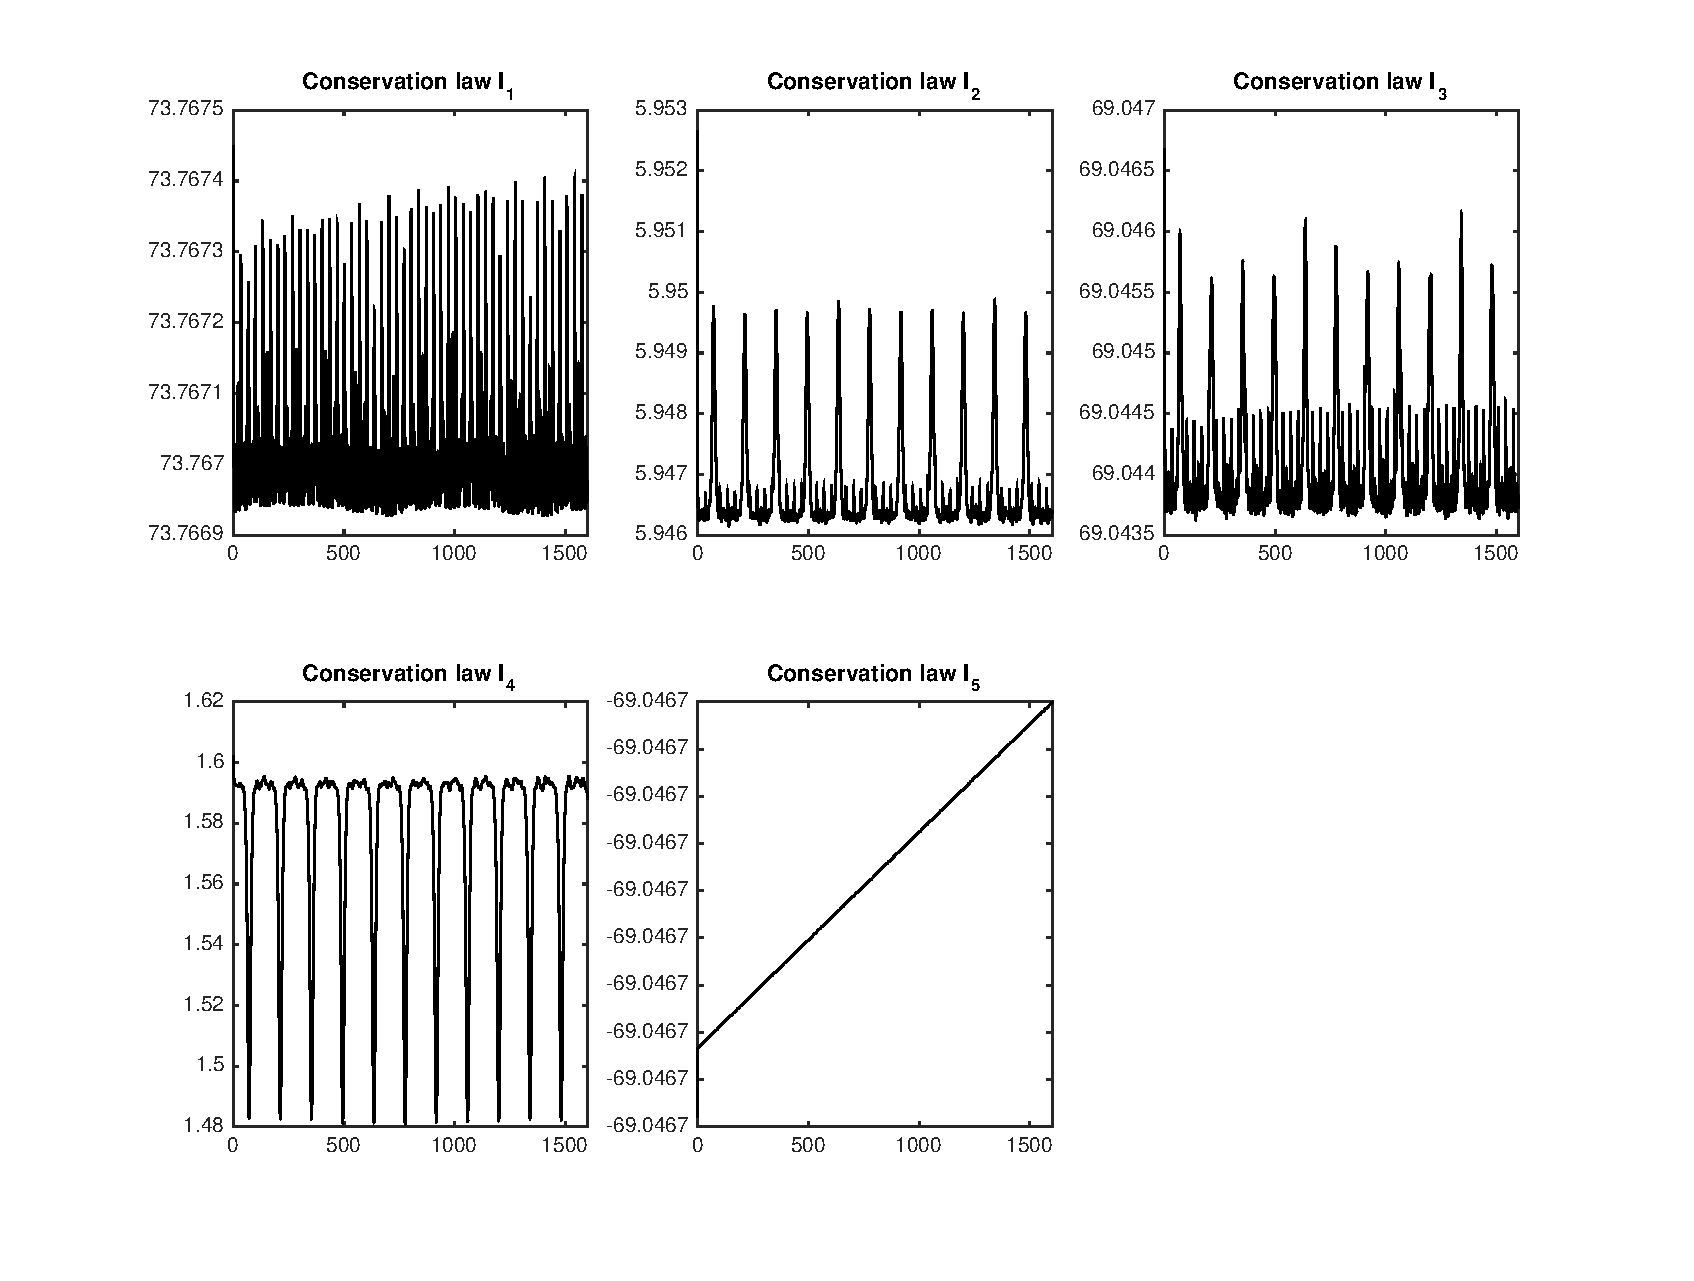
\includegraphics[width=\hsize]{conservation_laws}
%\caption{This plot shows the conservation laws of the deterministic Camassa-Holm equation, $H^1$ EPDiff, with linear dispersion. The initial condition is chosen to be two solitons with different amplitutes. }
%\end{sidefigureh}

%\printbibliography




\end{column}
\begin{column}{.31\textwidth}
\begin{block}{Discrete Clebsch Variational Principle}
\begin{itemize}
\item The constrained reduced Lagrangian is discretised $L_d $ and the derivatives are approximated using finite differences
\begin{align*}
L_d =&  \ell_d(u_i^n) \Delta t +  \pi_i^n \left( l_i^{n+1} - l_i^n  + \frac{u_i^n (l_{i+1}^n - l_{i-1}^n) + u_i^{n+1} (l_{i+1}^{n+1} - l_{i-1}^{n+1})}{4 \Delta x}  \Delta t  \right)  \\
&+ \sum_k \xi_i^k \left( \frac{l_{i+1}^n - l_{i-1}^n + l_{i+1}^{n+1} - l_{i-1}^{n+1}}{4 \Delta x} \right)  \Delta W_n^k, \quad  \Delta W_n^k \in \mathcal{N}(0, \Delta t)
\end{align*}
 \\
\item The discrete action is
\begin{align*}
\mathbb{S}_d = \sum\limits_{n=0}^{N_t-1}\sum\limits_{i=1}^{N_x-1} L_d & \left(  u_i^n, u_{i+1}^n, u_{i-1}^{n},  u_i^{n+1}, u_{i+1}^{n+1}, u_{i-1}^{n+1}, l_i^{n}, l_{i+1}^{n}, l_{i-1}^{n},  \right. \\
& \left. l_i^{n+1}, l_{i+1}^{n+1}, l_{i-1}^{n+1}, \pi_i^n  \right) 
\end{align*} \\
\item The stationary variations $0 = \delta \mathbb{S}_d$, yield a system of nonlinear equations
\begin{align*}
&D_{u,1} L_d + D_{u,2} L_d + D_{u,3} L_d + D_{u,4} L_d + D_{u,5} L_d + D_{u,6} L_d = 0, \\
&D_{\pi, 1} L_d = 0, \\
&D_{l,1} L_d + D_{l,2} L_d + D_{l,3} L_d + D_{l,4} L_d + D_{l,5} L_d + D_{l,6} L_d = 0 
\end{align*}
\end{itemize}
    \end{block}

\begin{block}{Publications}
\bibliographystyle{amsalpha}
\setbeamercolor{bibliography entry author}{fg=normal text.fg}
{\small \bibliography{refs}}
\end{block}

\end{column}
\end{columns}


\end{frame}
\end{document}